\subsection*{Menu} \label{sec:menu}

Menu is a lot more complicated than the HUD which is described in \autoref*{sec:hud}.
Because of that we decided to create a framework for creating menus.
This framework was heavily inspired by Flutter.
It uses the same concepts and terminology.
The overall idea is that everything is a widget.
A widget is a class that has a render method as well as a get size method.
Some widgets also have children so the overall structure of the menu is a tree of widgets.

An example of a widget is shown in \autoref*{fig:main_menu}.
This widget renders the main menu of the game.
The rendering logic of this widget can be seen in \autoref*{fig:widget_logic}.
The idea is as follows.
The root widget calls the render method of it's child which is the \texttt{Background} widget.

\begin{figure}
    \centering
    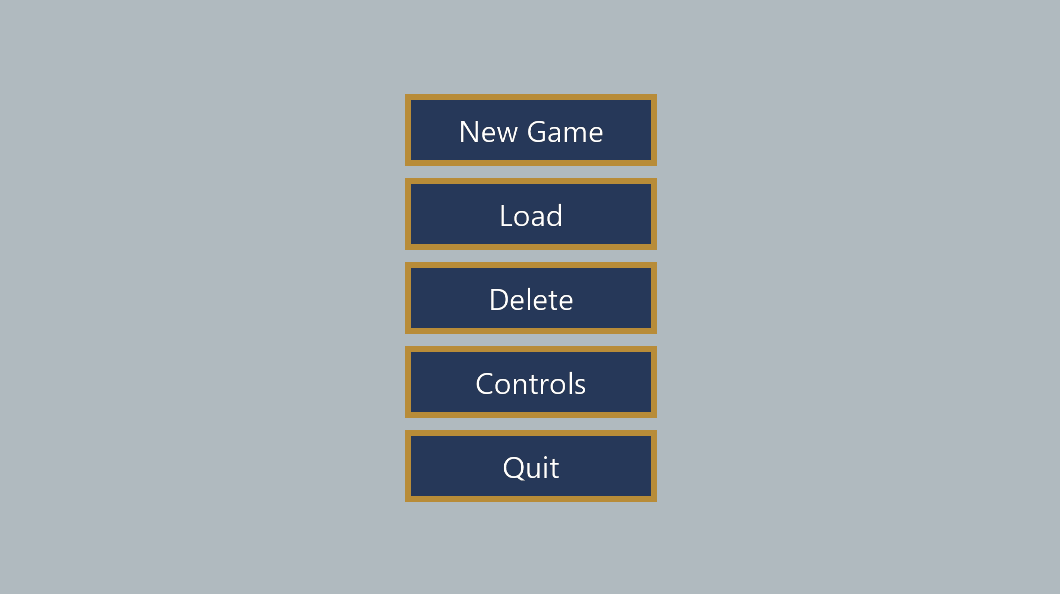
\includegraphics[width=0.8\textwidth]{chapters/two_dimensional_graphics/resources/main-menu.png}
    \caption{Main menu.}
    \label{fig:main_menu}
\end{figure}

\begin{figure}[H]
    \centering
    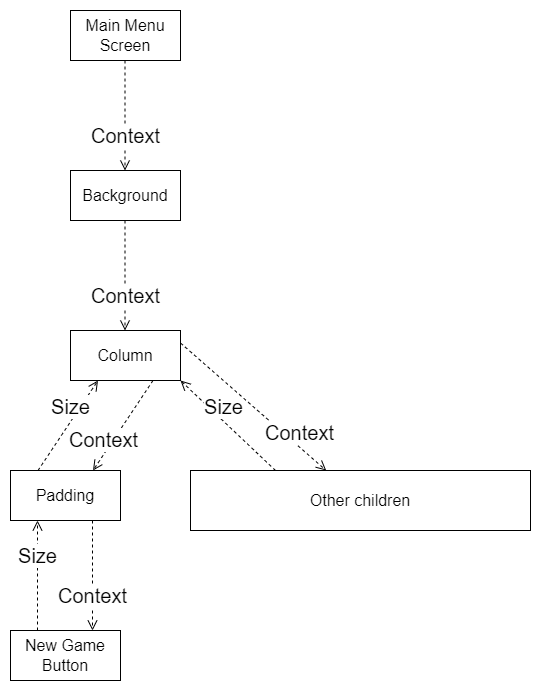
\includegraphics[width=0.8\textwidth]{chapters/two_dimensional_graphics/resources/widget_logic.drawio.png}
    \caption{Widget rendering logic.}
    \label{fig:widget_logic}
\end{figure}